\documentclass[11pt,letterpaper,twoside]{report}

% Layout
\usepackage{geometry}
\usepackage{setspace}
\usepackage{titlesec}
\usepackage[subfigure]{tocloft}

% Citation style
\usepackage{natbib}
\usepackage{apalike}

% include citations inline
\usepackage{bibentry}
\nobibliography*

% Figures
\usepackage{subfigure}
\usepackage{epsfig}
\usepackage{booktabs}
\usepackage{multicol}
\usepackage{listings}
\usepackage[table,xcdraw]{xcolor}

% Math
\usepackage{amsthm}
\usepackage{amsmath}
\usepackage{amssymb}
\usepackage{mathtools}
\DeclarePairedDelimiter{\ceil}{\lceil}{\rceil}

% Typography
\usepackage{times}
\usepackage{microtype}
\usepackage{textcomp}

% Macro support
\usepackage{xspace}

% PDF links
\usepackage[hidelinks]{hyperref} % backref=page

\usepackage{graphicx}
\graphicspath{{./figures/}}


% Use proper margins.
\geometry{letterpaper,left=1.25in,top=1in,right=1.25in,bottom=1in,nohead}



% double-space text
\doublespacing

% Center chapter titles, omit page numbers.
\titleformat{\chapter}[display]{\fillast\bfseries}{\Large\MakeUppercase{\chaptertitlename} \thechapter}{-11pt}{\huge\singlespacing}[\thispagestyle{empty}]

% Extend to 2in top margins
% Leave 22pts = 2x font size after heading
\titlespacing{\chapter}{0in}{0.62in}{22pt}

% Indent paragraphs four spaces throughout the thesis/dissertation.
\setlength{\parindent}{4ex}

% Tweak spacing of paragraph labels.
\titlespacing{\paragraph}{0in}{0.08in}{0.07in}

% We want numbered subsubsections
\setcounter{secnumdepth}{3}
\setcounter{tocdepth}{3}

% We need to double-space between footnotes.
\setlength{\footnotesep}{13pt}

% We don't want crazy vertical spacing.
\raggedbottom

% We don't want abandoned words.
\clubpenalty=10000 
\widowpenalty=10000

% Prevent awkward hyphenations.
\hyphenation{Raj-kumar}


% citation style

% default: cite with (Name, year)
\renewcommand{\cite}{\citep}

% common abbreviations
\newcommand{\eg}{{\it e.g.}\xspace}
\newcommand{\ie}{{\it i.e.}\xspace}
\newcommand{\etc}{{\it etc.}\xspace}
\newcommand{\etal}{\emph{et~al}\mbox{.}\xspace}

\newcommand{\xth}{\ensuremath{^{\text{th}}}\xspace}
%\newcommand{\fst}{\ensuremath{^{\text{st}}}\xspace}



\newcommand{\vs}{{vs\mbox{.}}\xspace}

% common Math notation
\newcommand{\NAT}[0]{\mathbb{N}\xspace}
\newcommand{\fun}[1]{\mathit{#1}} % typeset as function name
\newcommand{\setsize}[1]{\left| #1 \right|}
\newcommand{\setdef}[2]{\left\{ #1 \ \left|\  #2\right.\right\}}
\newcommand{\dispsum}[0]{\displaystyle\sum}

\newcommand{\defeq}[0]{\triangleq}
\renewcommand{\mod}{\operatorname{mod}}

% time units
\newcommand{\mus}[0]{\ensuremath{\mu s}\xspace}
\newcommand{\us}[0]{\ensuremath{\mu s}}
\newcommand{\ms}[0]{\ensuremath{\fun{ms}}\xspace}

% algorithm names
\newcommand{\kwfont}[1]{\textsf{#1}\xspace} %\small
% variable name
\newcommand{\var}[1]{\ensuremath{{\fun{#1}}}\xspace} %\small

%http://hstuart.dk/2007/08/03/programming-latex-%E2%80%94-writing-commands/
\newcommand{\mkkw}[2]{
	\newcommand{#1}[0]{\kwfont{#2}}
}

% fancy symbols and functions
\newcommand{\Alg}[0]{{\mathcal A}}
\newcommand{\Test}[0]{{\mathcal T}}
\newcommand{\Mach}[0]{{\mathcal M}}

\newcommand{\usum}[0]{u_{\mathrm{sum}}}
\newcommand{\umax}[0]{u_{\mathrm{max}}}
\newcommand{\umin}[0]{u_{\mathrm{min}}}
\newcommand{\utop}[0]{u_{\mathrm{top}}}

\newcommand{\esum}[0]{e_{\mathrm{sum}}}
\newcommand{\emax}[0]{e_{\mathrm{max}}}
\newcommand{\emin}[0]{e_{\mathrm{min}}}
\newcommand{\etop}[0]{e_{\mathrm{top}}}

\newcommand{\dsum}[0]{\delta_{\mathrm{sum}}}
\newcommand{\dmax}[0]{\delta_{\mathrm{max}}}
\newcommand{\dmin}[0]{\delta_{\mathrm{min}}}
\newcommand{\dtop}[0]{\delta_{\mathrm{top}}}

\newcommand{\prio}[0]{\mathsf Y}
\newcommand{\eprio}[0]{\mathsf y}

% src code
\newcommand{\src}[1]{\textsf{\small #1}\xspace}


% schedulers
\mkkw{\cfs}{CFS}

\mkkw{\edf}{EDF}
\mkkw{\edfwm}{EDF-WM}
\mkkw{\fp}{FP}
\mkkw{\fprm}{RM}
\mkkw{\fpdm}{DM}
\mkkw{\gedf}{G-EDF}
\mkkw{\gsnedf}{GSN-EDF}
\mkkw{\gfp}{G-FP}
\mkkw{\pedf}{P-EDF}
\mkkw{\pfp}{P-FP}
\mkkw{\cedf}{C-EDF}
\mkkw{\pssched}{PS}

\mkkw{\pfsched}{PF}
\mkkw{\pd}{PD}
\mkkw{\pds}{PD$^2$}
\mkkw{\cpds}{C-PD$^2$}

\mkkw{\jlfp}{JLFP}
\mkkw{\jldp}{JLDP}


% Plugins

\mkkw{\pfpgi}{P-FP-Rm}
\mkkw{\pfpdi}{P-FP-R1}
\mkkw{\pedfgi}{P-EDF-Rm}
\mkkw{\pedfdi}{P-EDF-R1}
\mkkw{\cedfiigi}{C2-EDF-Rm}
\mkkw{\cedfiidi}{C2-EDF-R1}
\mkkw{\cedfiiigi}{C6-EDF-Rm}
\mkkw{\cedfiiidi}{C6-EDF-R1}
\mkkw{\gedfgi}{G-EDF-Rm}
\mkkw{\gedfdi}{G-EDF-R1}

\mkkw{\cedfalldi}{C24-EDF-R1}

\mkkw{\capdsiigi}{C2-aPD$^2$-Rm}
\mkkw{\capdsiidi}{C2-aPD$^2$-R1}

\mkkw{\capdsiiigi}{C6-aPD$^2$-Rm}
\mkkw{\capdsiiidi}{C6-aPD$^2$-R1}

\mkkw{\gapdsgi}{G-aPD$^2$-Rm}
\mkkw{\gapdsdi}{G-aPD$^2$-R1}

\mkkw{\cspdsiigi}{C2-sPD$^2$-Rm}
\mkkw{\cspdsiidi}{C2-sPD$^2$-R1}

\mkkw{\cspdsiiigi}{C6-sPD$^2$-Rm}
\mkkw{\cspdsiiidi}{C6-sPD$^2$-R1}

\mkkw{\gspdsgi}{G-sPD$^2$-Rm}
\mkkw{\gspdsdi}{G-sPD$^2$-R1}


% POSIX

\mkkw{\schedfifo}{SCHED\_FIFO}
\mkkw{\schedrr}{SCHED\_RR}
\mkkw{\schedother}{SCHED\_OTHER}
\mkkw{\schedspor}{SCHED\_SPORADIC}
\mkkw{\prioprot}{PRIO\_PROTECT}
\mkkw{\scheddl}{SCHED\_DEADLINE}

% locking protocols
\mkkw{\npcs}{NCP}
\mkkw{\srp}{SRP}
\mkkw{\pcp}{PCP}
\mkkw{\msrp}{MSRP}
\mkkw{\dpcp}{DPCP}
\mkkw{\mpcp}{MPCP}
\mkkw{\mpcpvs}{MPCP-VS}
\mkkw{\fmlp}{FMLP}
\mkkw{\fmlpp}{FMLP$^{\mathrm{+}}$}
\mkkw{\npfmlpp}{NP-FMLP$^{\mathrm{+}}$}
\mkkw{\omlp}{OMLP}
\mkkw{\pip}{PIP}

% RW lock implementations
\mkkw{\pft}{PF-T}   % simple PF RW lock
\mkkw{\pfc}{PF-C}   % compact PF RW lock 
\mkkw{\pfq}{PF-Q}  % queue PF RW lock
\mkkw{\rwlin}{LX-RW}
\mkkw{\tft}{TF-T}
\mkkw{\tfq}{TF-Q}
\mkkw{\mtxt}{MX-T}
\mkkw{\mtxq}{MX-Q}

% locking protocol details
\newcommand{\FQ}[1]{FQ$_{#1}$}
\newcommand{\PQ}[1]{PQ$_{#1}$}

\newcommand{\WQ}[1]{WQ$_{#1}$}
\newcommand{\RQA}[1]{CQ$_{#1}$}
\newcommand{\RQP}[1]{DQ$_{#1}$}
\newcommand{\RQ}[2]{RQ$_{#1}^{#2}$}
\newcommand{\RQi}[1]{\RQ{#1}{1}}
\newcommand{\RQii}[1]{\RQ{#1}{2}}

\newcommand{\KQ}[1]{KQ$_{#1}$}
\newcommand{\KQq}[0]{\KQ{q}\xspace}
\newcommand{\RS}[1]{RS$_{#1}$}
\newcommand{\RSq}[0]{\RS{q}\xspace}

\newcommand{\BQ}[1]{BQ$_{#1}$}

\newcommand{\mc}[0]{\frac{m}{c}}
\newcommand{\nc}[0]{\frac{n}{c}}
\newcommand{\lmax}{L^{\fun{max}}}
\newcommand{\kmin}{k^{\fun{min}}}

% references
\newcommand{\chref}[1]{Chapter~\ref{ch:#1}\xspace}
\newcommand{\chrefs}[2]{Chapters~\ref{ch:#1} and~\ref{ch:#2}\xspace}
\newcommand{\secref}[1]{Section~\ref{sec:#1}\xspace}
\newcommand{\figref}[1]{Figure~\ref{fig:#1}\xspace}
\newcommand{\figrefi}[2]{Figure~\ref{fig:#1}(#2)\xspace}
\newcommand{\tabref}[1]{Table~\ref{tab:#1}\xspace}
\newcommand{\lemref}[1]{Lemma~\ref{lem:#1}\xspace}
\newcommand{\thmref}[1]{Theorem~\ref{thm:#1}\xspace}
\newcommand{\defref}[1]{Definition~\ref{def:#1}\xspace}
\newcommand{\exref}[1]{Example~\ref{ex:#1}\xspace}
\newcommand{\equref}[1]{Equation~(\ref{eq:#1})\xspace}
\newcommand{\inequref}[1]{Inequality~(\ref{eq:#1})\xspace}
\newcommand{\lstref}[1]{Listing~\ref{lst:#1}\xspace}
\newcommand{\pref}[1]{page~\pageref{p:#1}\xspace}
% citations

% resource notation
\newcommand{\res}[0]{\ell}
\newcommand{\req}[0]{\mathcal{R}}
\newcommand{\wreq}[0]{\mathcal{R}^{\fun{W}}}
\newcommand{\rreq}[0]{\mathcal{R}^{\fun{R}}}
\newcommand{\rlen}[0]{{\mathcal L}}
\newcommand{\bspin}[0]{s}

% locking proofs
\newcommand{\tauseq}[0]{\tau^{\fun{seq}}}

% overheads
\newcommand{\evlat}[0]{\Delta^{\fun{ev}}}
\newcommand{\ipilat}[0]{\Delta^{\fun{ipi}}}
\newcommand{\reloh}[0]{\Delta^{\fun{rel}}}
\newcommand{\schedoh}[0]{\Delta^{\fun{sch}}}
\newcommand{\cxsoh}[0]{\Delta^{\fun{cxs}}}
\newcommand{\cpmdoh}[0]{\Delta^{\fun{cpd}}}
\newcommand{\cidoh}[0]{\Delta^{\fun{cid}}}
\newcommand{\tickoh}[0]{\Delta^{\fun{tck}}}

\newcommand{\inoh}[0]{\Delta^{\fun{in}}}
\newcommand{\outoh}[0]{\Delta^{\fun{out}}}

\newcommand{\sysinoh}[0]{\Delta^{\fun{sci}}}
\newcommand{\sysoutoh}[0]{\Delta^{\fun{sco}}}


\newcommand{\numres}[0]{{n_r}}

% complicated names
\newcommand{\litmus}{LITMUS$^{\mathrm{RT}}$\xspace}
\newcommand{\aquo}{AQuoSA\xspace}
\newcommand{\prt}{PREEMPT\_RT\xspace}
\newcommand{\livlin}{L$^4$Linux\xspace}

% parameters

\newcommand{\pacc}[0]{\var{pacc}}
\newcommand{\wratio}[0]{\var{wratio}}

% special footnotes

% from http://help-csli.stanford.edu/tex/latex-footnotes.shtml
\long\def\symbolfootnote[#1]#2{\begingroup%
\def\thefootnote{\fnsymbol{footnote}}\footnote[#1]{#2}\endgroup}

% Theorems, etc.

\newtheoremstyle{mylemthm}% hnamei 
        {6pt}% hSpace abovei 
        {3pt}% hSpace belowi 
        {\slshape}% hBody fonti 
        {}% hIndent amounti1
        {\bfseries}% hTheorem head fonti 
        {.}% hPunctuation after theorem headi 
        {.5em}% hSpace after theorem headi2
        {}% hTheorem head spec (can be left empty, meaning `normal')i

\theoremstyle{mylemthm}

\newtheorem{theorem}{Theorem}[chapter]
\newtheorem{lemma}{Lemma}[chapter]

%\theoremstyle{definition}

\newtheoremstyle{mydef}% hnamei 
        {3pt}% hSpace abovei 
        {3pt}% hSpace belowi 
        {\normalfont}% hBody fonti 
        {}% hIndent amounti1
        {\bfseries}% hTheorem head fonti 
        {.}% hPunctuation after theorem headi 
        {.5em}% hSpace after theorem headi2
        {\thmname{#1} \thmnumber{#2}\thmnote{#3}}% hTheorem head spec (can be left empty, meaning `normal')i

\theoremstyle{mydef}


%% Flush words right at end of paragraph.
%% From: http://tex.stackexchange.com/questions/16330/hfill-after-linebreak
\newcommand\rightparend[1]{{%
      \unskip\nobreak\hfil\penalty50
      \hskip2em\hbox{}\nobreak\hfil\textbf{#1}%
      \parfillskip=0pt \finalhyphendemerits=0 \par}}


\newtheorem{definition}{Definition}[chapter]
\newtheorem{xxexample}{Example}[chapter]

%% "inherent" from xxexample, but place box at the end of example.
\newenvironment{example}{
\begin{xxexample}
}{
\rightparend{$\Diamond$}
\end{xxexample}
}
% \qed   \sqbullet \blackdiamond \vartriangleleft



\begin{document}

% Title page, TOC, etc.

% front matter pages use 2in top margin
\newgeometry{left=1.25in,top=2in,right=1.25in,bottom=1in,nohead}
\pagenumbering{roman}

%1. Title Page

\begin{titlepage}
\begin{center}

% 1. The title of the thesis/dissertation, centered 2� below the top of the page

\vspace{2in}
\begin{singlespace}
\Large 
ADAPTING COMMUNITY DETECTION APPROACHES TO LAGRE, MULTILAYER, AND ATTRIBUTED NETWORKS
\end{singlespace}


% 2. Your name, centered 1� below the title.
\vspace{61pt} % 1 in = 72pt, 11pt for the line with text
\large Natalie Stanley
\end{center}


%3. The following statement, within the full mar- gins, 1� below your name:
%�A dissertation [or thesis] submitted to the faculty of the University of North Carolina at Chapel Hill in partial fulfillment of the requirements for the degree of	in the Department [or School or Curriculum] of      .�

\vspace{50pt}
\begin{singlespace}
\noindent \large
A dissertation submitted to the faculty of the University of North Carolina at Chapel Hill
in partial fulfillment of the requirements for the degree of Doctor of Philosophy in
the Curriculum in Bioinformatics and Computational Biology.
\end{singlespace}


%4. On the lower half of the page, centered, the words �Chapel Hill�
%and one line below that, the year in which your committee approves
%the completed thesis/dissertation.
\vspace{50pt}
\begin{center}
\begin{singlespace} \large
Chapel Hill\\
2018
\end{singlespace}
\end{center}

%5. On the right-hand side of the page, �Approved by,� followed by lines for the
%signatures of the adviser and four (two for thesis) readers. List

\vspace{60pt}
\begin{flushright}
\begin{minipage}[t]{1.2in} \large
Approved by:\\
%To be approved by: \\
Peter Mucha \\
Marc Niethammer\\
Jeremy Purvis \\
Tamara Berg \\
David Gotz \\
Laura Miller 
\end{minipage}
\end{flushright}

\end{titlepage}

%2. Copyright Page (optional)
\newgeometry{left=1.25in,top=8.33in,right=1.25in,bottom=1in,nohead}

%If you wish to copyright your thesis, you must include a copyright page with the following information single-spaced and centered on the bottom half of the page:
%� Year 
%Full Name (exactly as it appears on the title page) 
%ALL RIGHTS RESERVED
%This page should immediately follow the title page, and should bear the lower case Roman numeral: ii.

\begin{center}
\begin{singlespace}
\copyright 2018\\
Natalie Stanley \\
ALL RIGHTS RESERVED
\end{singlespace}
\end{center}

\clearpage

\newgeometry{left=1.25in,top=2in,right=1.25in,bottom=1in,nohead}

%3. Abstract

% Normal pages from here on out; TOC title takes care of 2in requirement.
\restoregeometry

%The word �Abstract� should be centered 2? below the top of the page. 
%Skip one line, then center your name followed by the title of the 
%thesis/dissertation. Use as many lines as necessary. Centered below the 
%title include the phrase, in parentheses, �(Under the direction of  
%_________)� and include the name(s) of the dissertation advisor(s).
%Skip one line and begin the content of the abstract. It should be 
%double-spaced and conform to margin guidelines. An abstract should not 
%exceed 150 words for a thesis and 350 words for a dissertation. The 
%latter is a requirement of both the Graduate School and UMI's 
%Dissertation Abstracts International.
%Because your dissertation abstract will be published, please prepare and 
%proofread it carefully. Print all symbols and foreign words clearly and 
%accurately to avoid errors or delays. Make sure that the title given at 
%the top of the abstract has the same wording as the title shown on your 
%title page. Avoid mathematical formulas, diagrams, and other 
%illustrative materials, and only offer the briefest possible description 
%of your thesis/dissertation and a concise summary of its conclusions. Do 
%not include lengthy explanations and opinions.
%The abstract should bear the lower case Roman number ii (if you did not 
%include a copyright page) or iii (if you include a copyright page).

\begin{center}
\vspace*{52pt}
{\Large \textbf{ABSTRACT}}
\vspace{11pt}

\begin{singlespace}
Natalie Stanley: Adapting community detection approaches to large, multilayer, and attributed networks  \\
(Under the direction of Peter J. Mucha)
\end{singlespace}
\end{center}

Networks have become a common data mining tool to encode relational definitions between a set of entities. Whether studying biological correlations, or communication between individuals in a social network, network analysis tools enable interpretation, prediction, and visualization of patterns in the data. Community detection is a well-developed subfield of network analysis, where the objective is to cluster nodes into `communities' based on their connectivity patterns. There are many useful and robust approaches for identifying communities in a single, moderately-sized network, but the ability to work with more complicated types of networks containing extra or a large amount of information poses challenges. In this thesis, we address three types of challenging network data and how to adapt standard community detection approaches to handle these situations. In particular, we focus on networks that are large, attributed, and multilayer. First, we present a method for identifying communities in multilayer networks, where there exist multiple relational definitions between a set of nodes. Next, we provide a pre-processing technique for reducing the size of large networks, where standard community detection approaches might have inconsistent results or be prohibitively slow. We then introduce an extension to a probabilistic model for community structure to take into account node attribute information and develop a test to quantify the extent to which connectivity and attribute information align. Finally, we demonstrate example applications of these methods in biological and social networks. This work helps to advance the understand of network clustering, network compression, and the joint modeling of node attributes and network connectivity. 
\clearpage


%4. Dedication, Acknowledgement(s) and/or Preface (all optional)

%A dedication is an honorific statement from the author to a person or group to 
%whom the author commends the effort and product of the dissertation. Most 
%dedications are short statements of tribute beginning with �To��. No heading is 
%required on the dedication page. The text of short dedications should be 
%centered between the left and right margins and 2? from the top of the page.

\begin{center}
\vspace*{52pt}

To Thomas. Thank you for being you.  

\end{center}

\pagebreak

%Acknowledgements are the author's statement of gratitude to and
%recognition of the people and institutions who helped the author's
%research and writing.

\begin{center}
\vspace*{52pt}
{\Large \textbf{ACKNOWLEDGEMENTS}}
\end{center}

I'm glad this is the part of the thesis that people like to read because I have many thanks to share. First, thank you to my advisor, Peter. Thank you for always treating me like a scientist, and not a student. I think that a trait of a great advisor is their willingness to work collaboratively with their students, and Peter does this incredibly well. Thank you for always being positive about results (even if no positivity was warranted), for providing suggestions, and for allowing me to work on whatever I wanted to. Thank you for helping me through `existential angst' and for supporting me in whatever career path I wanted to take. Thank you for always making sure there was a grant to pay my salary and for all of the meetings and Slack conversations. I will forever remember to ignore the gong and how one good result is already more than most of the literature. I am forever grateful for all of your support.

Next, thank you to my pseudo second advisor, Marc. Thank you for always reading my write ups and papers and always having great questions and suggestions. I always admire how successful, creative, and humble you are (oh and a great sense of humor). Thank you for all of the time and Monday meetings. The Monday meetings with Peter and Roland are some of my best memories. 

Thank you to Saray and Dane who have played an important role in mentoring me as a beginning grad student and helping me to write my first paper. Dane, thank you for your very detailed editing and notation considerations. I will forever remember the suggestions you made on the first paper. Saray, I am so lucky to work with you and even more lucky to have you as a friend. I rarely have met people that I can communicate with through eye contact. Our entropy together made everything more fun, from yard time, to `getting a mix', to flying with the random physicist to Zarzagoza (said with the Spanish accent) and eating way too much at Weaver Street. 

Thank you to my committee members, Jeremy, Tamara, Laura and David. Jeremy, thank you for being my first introduction to research in grad school. I will always remember p53 signaling dynamics and microRNAs. Tamara, I am so happy that I got to take your class in my second year, which inspired me so much and even made me wish I could switch to computer vision. You are a great role model as a smart and creative researcher. Laura and David, thank you for all of your suggestions in committee meetings and for reading this thesis.

I have been lucky to interact with a lot of great people over the years in the Mucha research group. Thanks to Nishant, Wayne, Sam, Howdy, Clara, Eun, Peter D, Nic, and Sean for brightening up Chapman.

Thank you to the people who make BCB run- Tim Elston, Will Valdar, and John Cornett. I know you all work very hard for BCB and I think we have a great group of creative students. We all owe so much gratitude to John Cornett who is always friendly, positive, responsive, and on top of things. I am also lucky to have met great friends in BCB who I have done homework with, looked up to, and gotten advice from. Thank you, Bryan, Dan, Greg, and Paul. 

Thanks to living in Chapel Hill, I was fortunate to make some incredible friends. To my super strong (literally strong) lady friends Jess, Mimi, and Libby: Thank you for all the nights we spent laughing and climbing. These are some of the best times. Thank you Andrew for being the most incredible nerd friend and one of the kindest people I have ever met. I can always count on you for awesome conversation. 

Last but not least, I owe a huge amount of gratitude to my family. First to my parents Pat and Eric who have supported me every day of my life. They have never put any pressure on me to do anything and support all of my dreams unconditionally. Most importantly, they are really friendly and fun people. I couldn't choose better parents. Thank you for tolerating my un responded text messages, my inability to mail a letter or find a stamp, and for helping me through tough times. Next to my brother, Mike. I admire you so much for always following your dreams and doing what feels right to you. Aside from being great at everything you do, you are such a kind, wonderful person. I hope you don't find any mistakes in this thesis or ask about consistency. 

Finally, thank you Thomas for supporting me in every possible way. I'm so happy that grad school lead me to you. You have enhanced my life in every way and inspire me every day to be a scientist. I am so lucky to have a great role model who works so hard, is so talented, and so kind. Thank you for always pushing me pursue things I didn't think that I could. Thank you for always telling me `shhhhhhh' when I started to get stressed. You are my favorite Dub.

OK, this is the end. Thank you everyone that read to the end.   

\clearpage


%\begin{center}
{\Large \textbf{PREFACE}}
\end{center}

Suspendisse semper, nibh at dignissim volutpat, nibh lacus tempus augue, nec tempus est leo nec sem. Phasellus eros felis, malesuada nec, lobortis quis, posuere in, risus. Cras sagittis accumsan purus. Nullam nulla nisl, ultrices a, lacinia eu, lacinia vitae, risus. Donec varius lorem. Nam nisl. Vivamus non augue. Vestibulum dignissim auctor neque. Ut vel eros. Aenean tempor, erat vel feugiat porta, nunc justo euismod dui, ut hendrerit dolor lusto sit amet tortor. Nunc adipiscing massa in erat. Proin tincidunt tellus vitae augue consequat suscipit. Aliquam feugiat libero non odio. Fusce adipiscing augue ac arcu. In orci. Cras lobortis euismod libero.
\tbw


\clearpage





%5. Table of Contents, with page references
\renewcommand{\contentsname}{TABLE OF CONTENTS}
\renewcommand{\cfttoctitlefont}{\hfill\Large\bfseries}
\renewcommand{\cftaftertoctitle}{\hfill}
\renewcommand{\cftdotsep}{1.5}
\cftsetrmarg{1.0in}

\setlength{\cftbeforetoctitleskip}{61pt}
\setlength{\cftaftertoctitleskip}{28pt}

% format chapter entries like other entries
\renewcommand{\cftchapfont}{\normalfont}
\renewcommand{\cftchappagefont}{\normalfont}
\renewcommand{\cftchapleader}{\cftdotfill{\cftdotsep}}

\setlength{\cftbeforechapskip}{15pt}
\setlength{\cftbeforesecskip}{10pt}
\setlength{\cftbeforesubsecskip}{10pt}
\setlength{\cftbeforesubsubsecskip}{10pt}

\begin{singlespace}
\tableofcontents
\end{singlespace}


\clearpage



%6. List of Tables, with titles and page references (if applicable)

\renewcommand{\listtablename}{LIST OF TABLES}
\phantomsection
\addcontentsline{toc}{chapter}{LIST OF TABLES}

\setlength{\cftbeforelottitleskip}{-11pt}
\setlength{\cftafterlottitleskip}{22pt}
\renewcommand{\cftlottitlefont}{\hfill\Large\bfseries}
\renewcommand{\cftafterlottitle}{\hfill}

\setlength{\cftbeforetabskip}{10pt}

\begin{singlespace}
\listoftables
\end{singlespace}

\clearpage



%7. List of Figures or Illustrations, with titles and page references (if applicable)

\renewcommand{\listfigurename}{LIST OF FIGURES}
\phantomsection
\addcontentsline{toc}{chapter}{LIST OF FIGURES}

\setlength{\cftbeforeloftitleskip}{-11pt}
\setlength{\cftafterloftitleskip}{22pt}
\renewcommand{\cftloftitlefont}{\hfill\Large\bfseries}
\renewcommand{\cftafterloftitle}{\hfill}

\setlength{\cftbeforefigskip}{10pt}
\cftsetrmarg{1.0in}

\begin{singlespace}
\listoffigures
\end{singlespace}
\clearpage


%8. List of Abbreviations (if applicable)
\phantomsection
\addcontentsline{toc}{chapter}{LIST OF ABBREVIATIONS}

\begin{center}
{\Large \textbf{LIST OF ABBREVIATIONS \& COMMON NOTATION}}
\end{center}

\newcommand{\Ab}[2]{\noindent  #1 \> #2 \\}
\newcommand{\Abi}[2]{\noindent #1 \hspace{1.5cm} \= #2 \\}

\begin{tabbing}
\Abi{SBM}{Stochastic Block Model}
\Ab{EM}{Expectation Maximization}
\Ab{sMLSBM}{Strata Multilayer Stochastic Block Model}
\Ab{MLSBM}{Multilayer Stochastic Block Model}
\Ab{${\bf A}$}{Network adjacency Matrix}
\Ab{$a_{ij}$}{The $ij$th entry of adjacency matrix, {\bf A}}
\Ab{SN}{Super Node}
\Ab{${\bf z}$}{For a network with $N$ nodes, this is the length $N$ vector of node-to-community assignments}
\Ab{$z_{i}$}{The community assignment of node $i$}
\Ab{${\bf Z}$}{The indicator matrix of node-to-community assignments}
\Ab{$z_{ik}$}{A binary indicator of whether node $i$ belongs to community $k$.}
\Ab{ALI}{Acute lung injury}
\Ab{OTU}{Operational taxonomic unit}
\Ab{DAG}{Directed acyclic graph}
\Ab{MCMC}{Markov Chain Monte Carlo}
\Ab{$p_{\text{in}}$}{Within-community edge probability under stochastic block model}
\Ab{$p_{\text{out}}$}{Between-community edge probability under stochastic block model}
\Ab{LP}{Label propagation}

\end{tabbing}

\clearpage


%9. List of Symbols (if applicable)

\pagenumbering{arabic}


% chapters
% \input{intro/chapter}
% ...

\chapter{Introduction}
Network data appears widely across fields as a data structure for modeling relational information between a set of entities.  In recent years, networks have become an indispensable data mining tool, as they allow for tasks such as, data visualization, clustering, and predictive modeling.  Motivated by problems in fields, such as, biology, medicine, neuroscience, social science, and epidemiology, the field of network analysis has gained popularity and seeks to develop tools for understanding the associated network data. The development of these tools is rooted in a combination of techniques from statistics, computer science, physics, and mathematics. In this thesis, we will provide a comprehensive overview of networks and analysis techniques and introduce three new models/methods that will expand the types of network data that we asre able to collect and interpret. 

\section{Network Notation}

\subsection{Representing relational information}

Humans frequently benefit from network applications for tasks such as, viewing relevant queries from a google search, enjoying a suggested movie on Netflix, or interacting on a social network platform. The basic building blocks of networks are nodes, representing entities in a systems, and edges, encoding connections their physical or inferred connection or similarity. Figure \ref{fig:social} shows a social network between 7 users and edges between them denoting whether they interact. 
\begin{figure}
\begin{center}
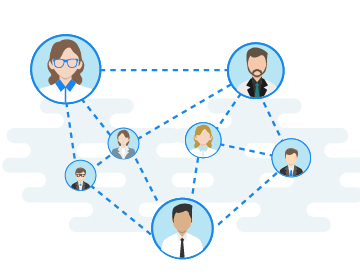
\includegraphics[scale=0.5]{SocialNetwork}
\caption{{\bf Toy social network.} A small example of a social network, with nodes being users and edges representing connections between users. Image from \url{https://www.phpfox.com}}
\label{fig:social}
\end{center}
\end{figure}

Such a network with edges simply representing whether or not a pair of nodes interact is an example of an \emph{undirected,unweighted} network. We will use an undirected network to introduce two forms of representations for networks. For a set of $N$ nodes, we define the $N \times N$ network adjacency matrix, ${\bf A}=\{a_{ij}\}$. For a pair of nodes $i$ and $j$, its corresponding adjacency matrix entry $a_{ij}$ is defined as follows,

\[ \begin{cases} 
     a_{ij}=1 & \text{\emph{if node $i$ and node $j$ are connected}} \\
      a_{ij}=0 & \text{\emph{otherwise}}.
         \end{cases}
\].

Undirected networks can also be \emph{weighted}, where the weight of an edge between a node pair encodes their extent of similarity. These edge weights are some real number and are frequently quantities such as correlation or pairwise similarity. A simple extension of ${\bf A}$ to an undirected, weighted network where $w$ is the edge weight between nodes $i$ and $j$ computes the adjacency matrix entry $a_{ij}$ as, 

\[ \begin{cases} 
     a_{ij}=w & \text{\emph{if node $i$ and node $j$ are connected} with weight $w$} \\
      a_{ij}=0 & \text{\emph{otherwise}}.
         \end{cases}
\]

Alternatively, the assumption of a symmetric relationship between a pair of nodes that node $i$ connects to node $j$ and node $j$ connects to node $i$  may be unrealistic. For example, on twitter, user $i$ can follow user $j$, but user $j$ does not necessarily need to follow user $i$. This type of network is known as a \emph{directed} network. While directed are frequently discussed in the network science literature, we will not introduce them here.  

\subsection{Basic Analysis}
Given a network, there are fundamental tasks of interest that allow for a more clear interpretation and understanding of the data. Some of these objectives include, quantifying node importance, quantifying edge density, identifying connected components ,clustering nodes, and predicting links. Networks in textbooks often look deceptively clean and well-structure. In reality, most network data is described as being a hairball. This term refers to the difficulty of discerning structure or interpreting meaning from the network based on the connectivity patterns. An example of a typical hairball is shown in figure \ref{fig:Hairball}

\begin{figure}
\begin{center}
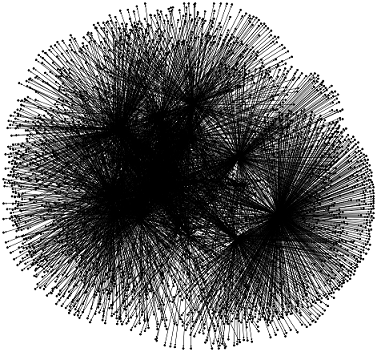
\includegraphics[scale=0.3]{Hairball}
\caption{{\bf Hairball network.} Networks are often noisy data structures and lack an immediate straight forward structural interpretation. Image from \url{https://cs.umd.edu}}
\label{fig:Hairball}
\end{center}
\end{figure}

Such a challenging representation of the data requires breaking the network down into smaller pieces that can be further analyzed. The first most basic summary statistic is known as \emph{degree}. Here, we will define a variety of summary statistics and quantities that can be computed on a network that give insight into the network's structure. Given the adjacency matrix for an undirected network, ${\bf A}$, the degree of node $i$, $\text{degree}(i)$ is computed as,

\begin{equation}
\text{degree}(i)=\sum_{j}a_{ij}
\end{equation}

In the case of an undirected, unweighted network, the degree of node $i$ counts its number of neighbors, while in the undirected, weighted context, degree encodes the total edge weight incident to node $i$. Collectively examining the distribution of degrees for a network is known as the \emph{degree distribution}. Understanding the degree distribution provides insight into the network type and structural organization. [Add some example maybe]. To concisely summarize this information, one may consider. ... blah blah to add. Finally, clustering on a network or identifying a partition of nodes into groups or `communities' based on structural network patterns is known as community detection. This is a powerful way to segment a network into smaller structures that can be further prioritized for additional analysis. 

\section{Conceptual Overview of Community Detection}
A community in a network is broadly defined as a set of who share something in common in terms of their connectivity patterns in the network. One can think of a community as a clustering problem on networks, where the objective is to identify a set of nodes that are highly similar. The most basic type of community to understand is a network with assortative community structure. In this case, nodes are tightly connected to each other but more sparsely connected to the rest of the network. An example of a network with assortative community structure is shown in \ref{fig:Assort.} Communities in the network are outlined with pink dotted lines.

 \begin{figure}
\begin{center}
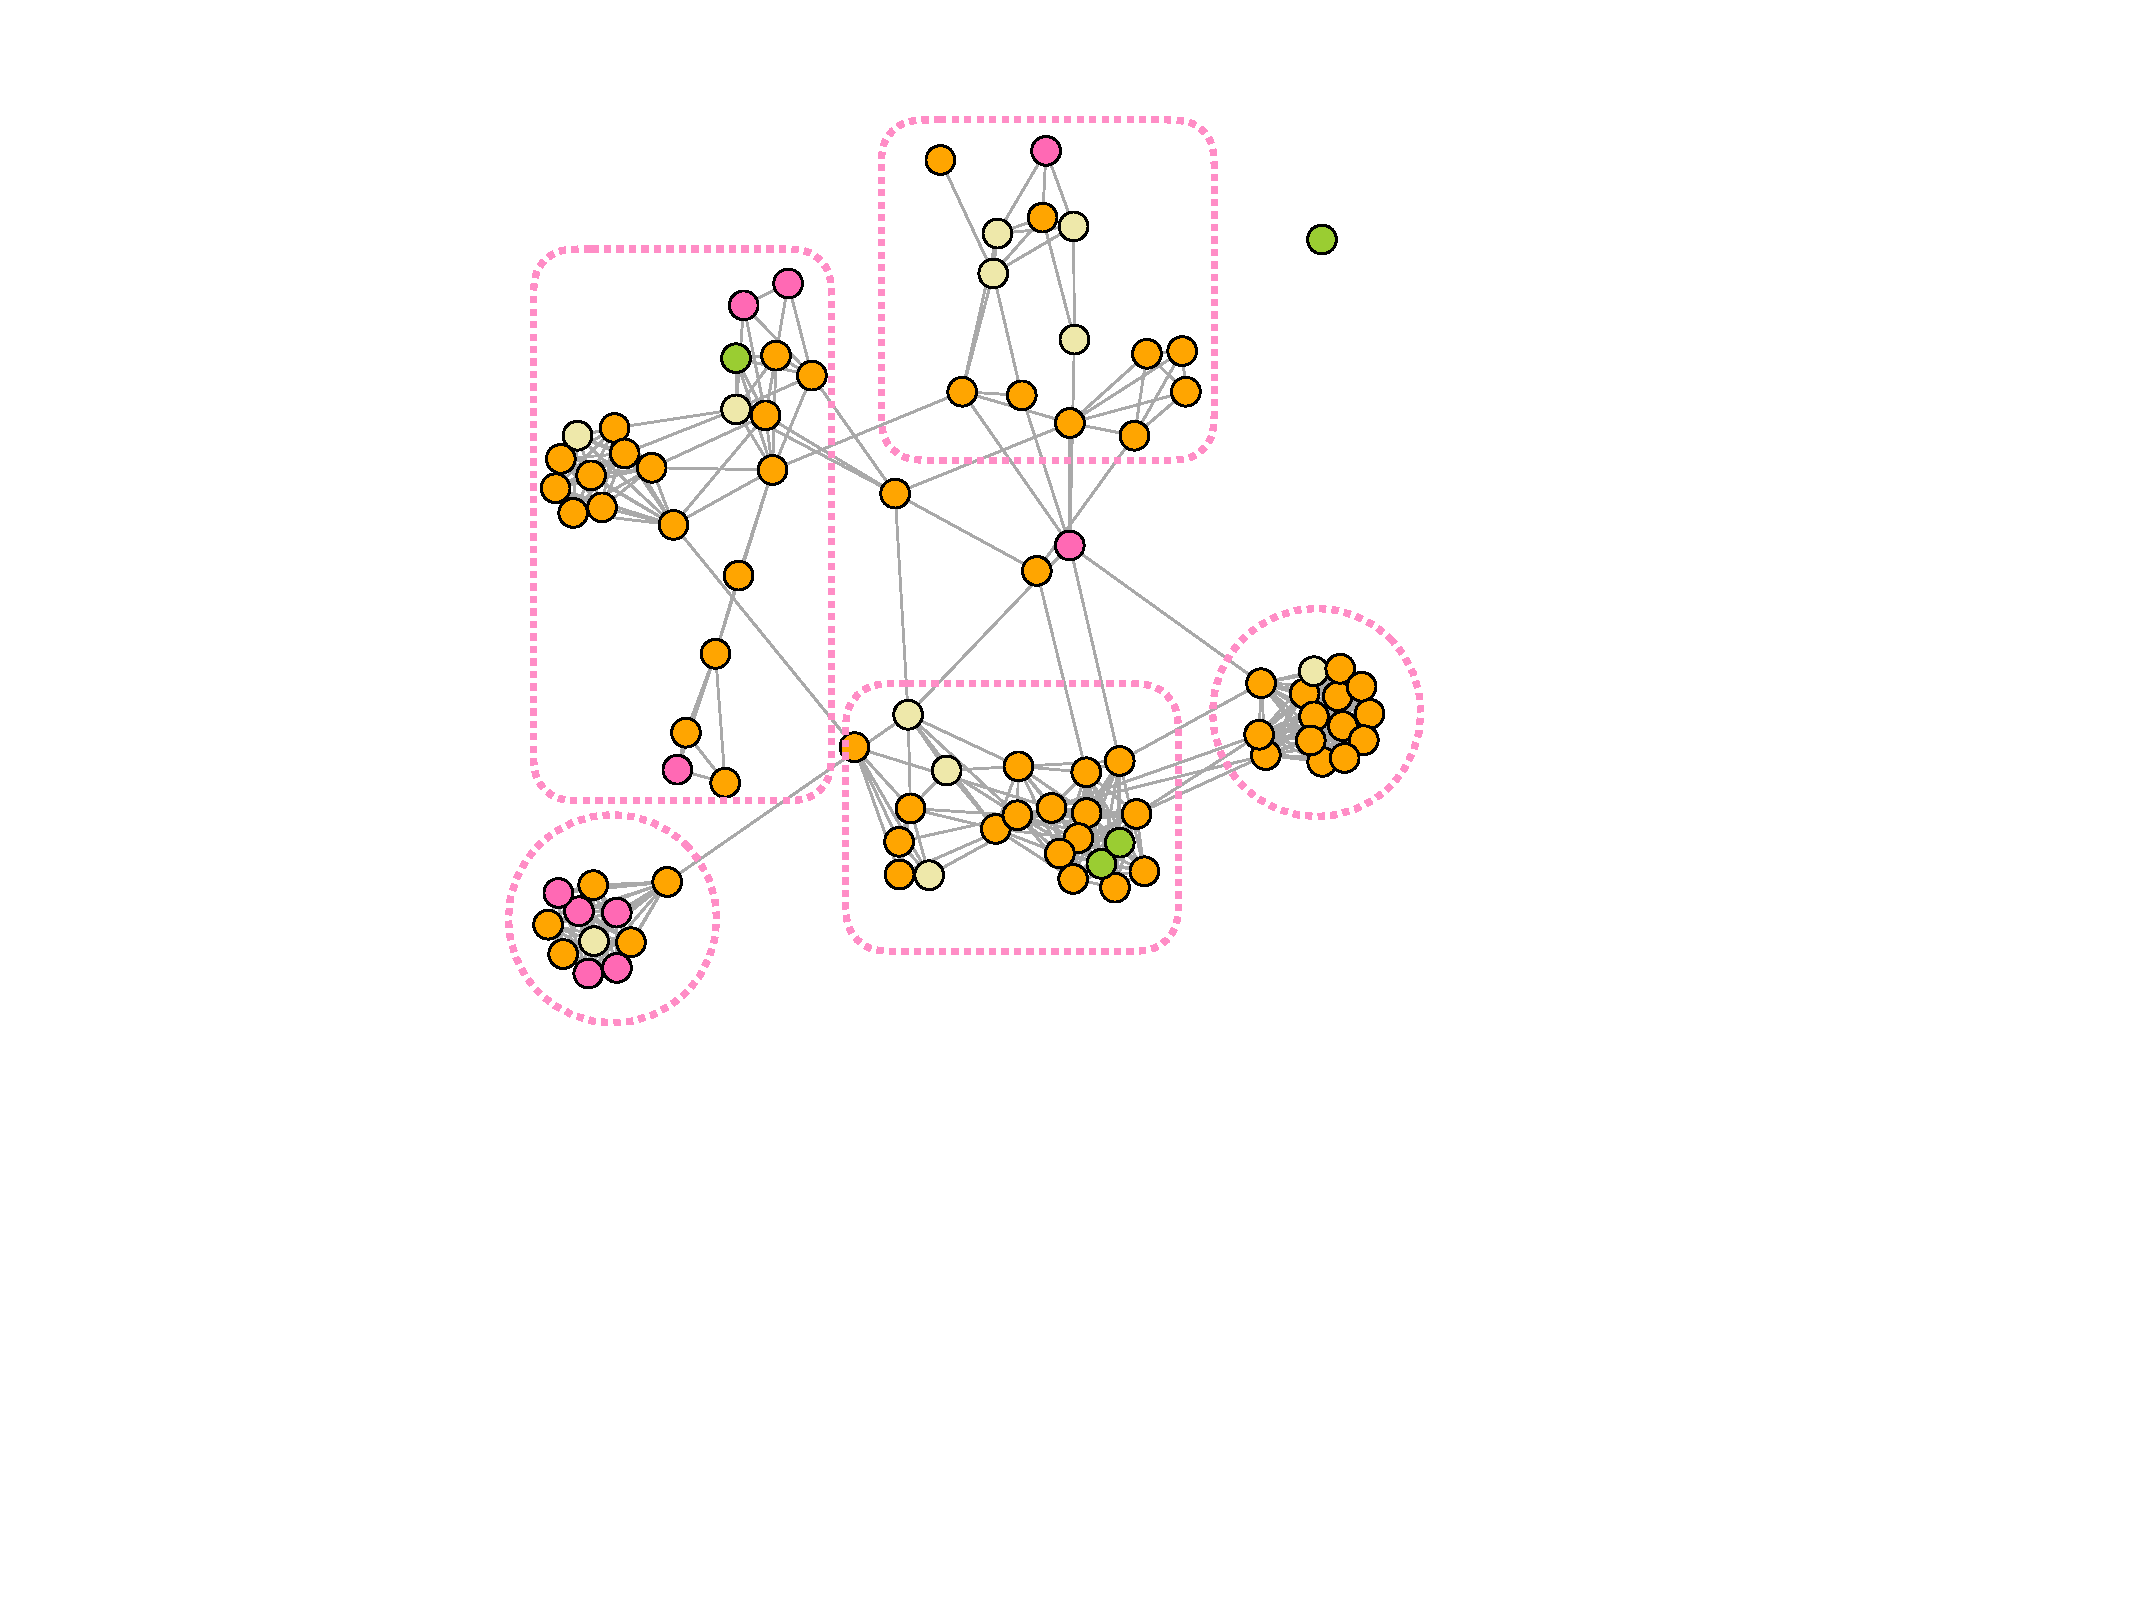
\includegraphics[scale=0.4]{AssortativeNet}
\caption{{\bf Assortative Community Structure.} Nodes are tightly connected to each other and more sparsely connected to the rest of the network. Each community is outlined with a pink dotted line.}
\label{fig:Assort}
\end{center}
\end{figure}

Alternatively, networks can have a dissasortative structure where the between community edge density exceeds the within-community density. Finally, a core periphery structure can arise when there is a central core in the network that connects to the rest of the network and a set of peripheral nodes that connect to the core, but not to each other.  

Community detection is a well-studied sub-domain of network science. The interested reader can refer to one of the comprehensive review articles \cite{fortu1,fortu2,shaicase}

\section{The state of the art methods}
When performing community detection on a network, the objective is to segment nodes into one of $K$ communities. This $K$ can be known apriori or estimated through some kind of model selection or quality function computations. There are many optimization approaches that can be used to approach network community detection. In this section, we will introduce the current state-of-the-art approaches characterized as quality function maximization, deep learning, higher order clustering, probabilistic, and spectral methods. These methods are discussed based on their ability to handle networks of non-trivial size with diverse structures.

\subsection{Quality function maximization with modularity}
\indent For quality function optimization, one writes down a quantity to optimize that seeks to identify a partition of the network into nodes that is representative of the network structure. The most common quality function for this task is known as modularity \cite{newman2006modularity}. Intuitively, modularity defines a null model for network that doesn't have prominent organizational structure. In particular, this null model is a random graph model, known as the configuration model \cite{benderCanfield}. To generate an $N$-node network from the configuration model, one first specifies a fixed degree sequence, $D=\{k_{i},k_{2},\dots,k_{N}\}$. From this sequence, nodes are connected with $k_{i}$ stubs that will ultimately be connected together. Finally, the graph is constructed by randomly choosing pairs of the crreated stubs and joining them. Based on how this network was generated, it is easy to specify the probability that an edge exists between a pair of nodes, $i$ and $j$, or $p(a_{ij}=1$.

\begin{equation}
p(a_{ij}=1)=\frac{k_{i}k_{j}}{2M}.
\end{equation}

Here, $k_{i}$ and $k_{j}$ represent the number of edges for nodes $i$ and $j$, respectively, and $M$ is the total number of edges in the network. 

\indent Modularity was introduced in 2004 by Newman and Girvan \cite{newmangirvan}. We define the modularity quality function, $Q$ as,

\begin{equation}
Q=\frac{1}{2M}\sum_{i,j}\left[a_{ij}-\gamma \frac{k_{i}k_{j}}{2M}\right]\delta(z_{i},z_{j})
\end{equation} 

Here, $\gamma$ is a resolution parameter \cite{resParam} that controls the scale of community size. Large values of $\gamma$ favor more small communities while smaller value enforce for fewer large communities. 

\indent In order to determine ${\bf z}$, the most computationally efficient approach is known as the Louvain algorithm \cite{blondel}. The Louvain algorithm is an agglomerative heuristic, which initially starts with each node in its own community and in the first match merges pairs of nodes if their merge leads to an increase in modularity. Each group of nodes assembled after this first pass becomes a new node in the network and a new weighted network is created between the set of new nodes. The weight on the edges of the new network are the number of edges from the original network that go between the sets of merged nodes. This process is continues iteratively until the modularity no longer increases. The reason that this approach is so computationally tractable is because the gain in modularity, $\Delta Q$ of merging two groups of nodes can be explicitly computed in closed form.

\indent Modularity has shown to be effective in applications from neuroscience \cite{hierarchicalmod} to image segmentation \cite{browet}.

\subsection{Identifying communities with probabilistic approaches}

\indent This approach will be only briefly introduced here, as it will be explored more in depth in subsequent chapters. Probabilistic community detection methods aim to find a partition of the network through likelihood optimization. Intuitively, the goal is to study the generative process of the node edges in terms of inferred community assignments. For example, given nodes $i$ and $j$, one may model $P(a_{ij}=1)$ as $g(z_{i},z_{j})$, where $g(\cdot)$ is some rule based on the node-to-community assignments. Two common probabilistic community detection models are the stochastic block model \cite{originalSBM} and the affiliation model \cite{affil}. The definition and description of these models and inference techniques are described in depth in chapter \ref{probTech}.

\subsection{Deep Learning Approaches}
\indent In recent years, deep learning has begun to revolutionize many fields, including network analysis. Perozzi \emph{et al.}, pioneered the use of deep learning in community detection with the development of DEEPWALK \cite{deepWalk} to learn a latent space representation of nodes in a lower dimensional space (i.e. an emedding). Once the network is embedded in a lower dimensional space, simple clustering techniques, such as $k$-means \cite{kMean} can be used to partition the network into communities. The approach to learn an embedding for the network is based on random walks on the network \cite{rWalk,gleichpagerank}. A random walk on a network involves choosing a starting node and traversing the network by hopping between adjacent nodes. The DEEPWALK approach seeks to learn an embedding of the nodes that preserves the sets of nodes traversed in a random walk. To do this, the authors used Word2Vec, a tool from natural language understanding that allow for the specification of a node embedding that enable accurate prediction of a word's context, given the word \cite{word2Vec}. To adapt this context to networks, a random walk is treated as a sentence and nodes are treated as a word within the sentence. Moreover, the analogous task to the problem in text data to a network is to accurately assign a probability predict a set of nodes likely to be seen with the node of interest. Moreover, this problem is solved using the same optimization approach as Word2Vec \\
\indent Based on the success of DEEPWALK, the method was followed up with Node2Vec in 2016 \cite{node2vec}. While node2vec also uses the random walk framework to specify the optimization problem, they modify how the random walk is performed to enable an embedding that captures different aspects of a potential network community. For example, one may describe a community by a set of nodes located close to each other in the network with many common neighbors and connections to common neighbors. This assumption is known as network homohpily \cite{homophily}. Alternatively, perhaps a good definition of a community is a set of networks that have similar roles in the network. This idea is known as structural equivalence \cite{structural}. For example, a grouping of nodes that take into account their degree, with the community assignments being highly related to node degree. To modify the random walk so that it leads to a model that gives flexibility in the nature of retrieved communities, the authors introduced a search bias term, which controls whether the random walk in performed in a breadth-first or depth-first search parameter. If on a random walk, the path is traversed in a depth-first search, favoring the exploration of a larger area of the network far from the source, the resulting community aligns with the homophily hyptohesis. A random walk performed in a breadth first manner that restricts the path to nodes neighboring the source and tends to capture nodes based on structural equivalence (i.e. a hub, or highly connected node). 

\section{Case studies in network community detection}
 A community approach to network analysis has shown to be fruitful in particular, in the analysis of biological and brain connectivity applications. In this section, we will describe examples of analyses where the identification of communities provided insight and understanding for a scientific problem. 
\subsection{Network analysis in computational biology}
Multiple experimental modalities exist that enable the collection and analysis of biological data. Understanding protein expression, gene expression, microbiome composition, metabolomic profiles, genomic mutations, and immune profiling are just a few of examples of biological data that is studied routinely for insight into human health. With most experimental platforms producing high dimensional data, it is crucial to have good tools for interpretation, visualization, and prediction. Machine learning techniques in computational biology have revolutionized prediction in healthcare and medicine. Here, we outline particular examples of how community detection lead to important biological understanding and predictive ability.

{\bf Immunological profiling to establish a pregnancy immune clock}
A study lead by Aghaeepour \emph{et al.}, demonstrated that there is a typical timing of immunological events in a healthy, term, human pregnancy \cite{immuneClock}. Immunological profiling was performed on a training cohort of 18 women, using a technology called mass cytometry \cite{cytof} was used to quantify various features of the immune system, such as, cell type abundances, signaling activity. From this set of measured immune features, a correlation network from the training cohort to identify which immune features were potentially related or working together. Simultaneously, a regression model was training to identify immune features associated with increased gestational age. When communities were identified in the network of immune features, there were two important observations. First, immune features of the same type (i.e. cell signaling vs. cell frequency) were aligned with community labels. Second, sets of features associated with a particular gestation age often fell in the same community, indicating their synchronous activity during the pregnancy. Finally, after identifying influential nodes in their ability to predict stage in pregnancy, according to the regression model, the communities of these nodes were more closely examined to uncover further insight into the immunological mechanisms occuring throughout the pregnancy time course. 



\section{Network analysis in neuroscience}




\section{Network analysis software}
\section{Open problems in community detection}

\section{Probabilistic graphical models for statistical inference}
\label{pgm}
Probabilistic network models are one approach to community detection that seek to model edge existence based on the node-to-community assignments. In doing so, the objective is to learn the node-to-community assignments that make the structure of the observed network the most likely. In this section, we will define some useful notation and concepts  To fit a probabilistic network model to data, we will define some useful notation and concepts that help simplify writing down and interpreting the likelihood. 

Probabilistic graphical models enable efficient specification and manipulation of large probability distributions through semantic structures. Given a set of random variables, $\{A,B,C,D,E,F\}$, we seek to compute the joint distribution, $P(A,B,C,D,E,F)$. This joint distribution can be expressed with a directed acyclic graph (DAG), whose structure encodes dependencies between random variables. The DAG allows for the representation of the joint distribution in a factorized way, which is computationally useful. A DAG between the set of random variables, $\{A,B,C,D,E,F\}$ is shown in \ref{fig:DAG}. 

\begin{figure}
\begin{center}
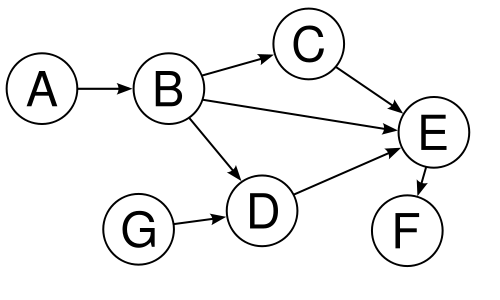
\includegraphics[scale=0.3]{DAG}
\caption{{\bf Directed Acyclic Graph.} A directed acyclic graph (DAG) is formed based on dependency between random variable and allows for a fully factorized probability distribution.}
\label{fig:DAG}
\end{center}
\end{figure}

To translate a DAG between a set of $N$ random variables, ${\bf X}={\bf X}=\{X_{1},X_{2},\dots,X_{N}\}$ to its joint distribution, we rely on the Factorization theorem, which specifies that a DAG factors according to its parent/child relationships with,

\begin{equation}
P({\bf X})=\prod_{i=1:N}P(X_{i} \mid {\bf X}_{\pi_{i}}).
\end{equation}

Here, ${\bf \pi}_{i}$ denotes the set of parents for node $i$. Using this information, we can write down the joint distribution for figure \ref{fig:DAG} as,

\begin{equation}
\begin{split}
P(A,B,C,D,E,F)&=P(A)P(B\mid A)P(C\mid B)P(D \mid B,G)P(E \mid D,B,C)P(F\mid E).
\end{split}
\end{equation}

This introduced idea will help in subsequent sections to expresses a model graphically, write down the model likelihood, and use the likelihood to optimize for the most appropriate model parameters. 


\chapter{Probabilistic community detection models and inference techniques}
\label{probTech}
In this section, we will present two probabilistic models for community structure, the stochastic block model and the affiliation model. 
\section{Stochastic block model}

\subsection{Most general stochastic block model}
For an undirected, unweighted network $\mathcal{G}$ with adjacency matrix, ${\bf A}$, we seek to partition each of the $N$ nodes into one of $K$ communities. We denote the the node-to-community assignments as ${\bf z}$, with $z_{i}$ specifying the community assignment of node $i$. Here, ${\bf z}$ is a latent variable, with each entry taking on 1 of $K$ states, or one of $K$ community assignments. Figure \ref{fig:graphical} shows the dependency relationship between the node-to-community assignments. Here, the node-to-community assignments are treated as a latent variables because we seek to identify the ${\bf z}$ that makes the observed adjacency matrix, ${\bf A}$ the most likely.  The crucial assumption of the stochastic block model is that nodes within a community are connected to nodes within their community and to other communities in a characteristic way. To this end, the model fitting procedure requires learning a set of within and between community connection probabilities. Under this approach, edges are treated as independent and identically distributed and deciding whether or node an edge exists between a pair of nodes is the learned connection probability between the communities to which each of the nodes belong.

\begin{figure}
\begin{center}
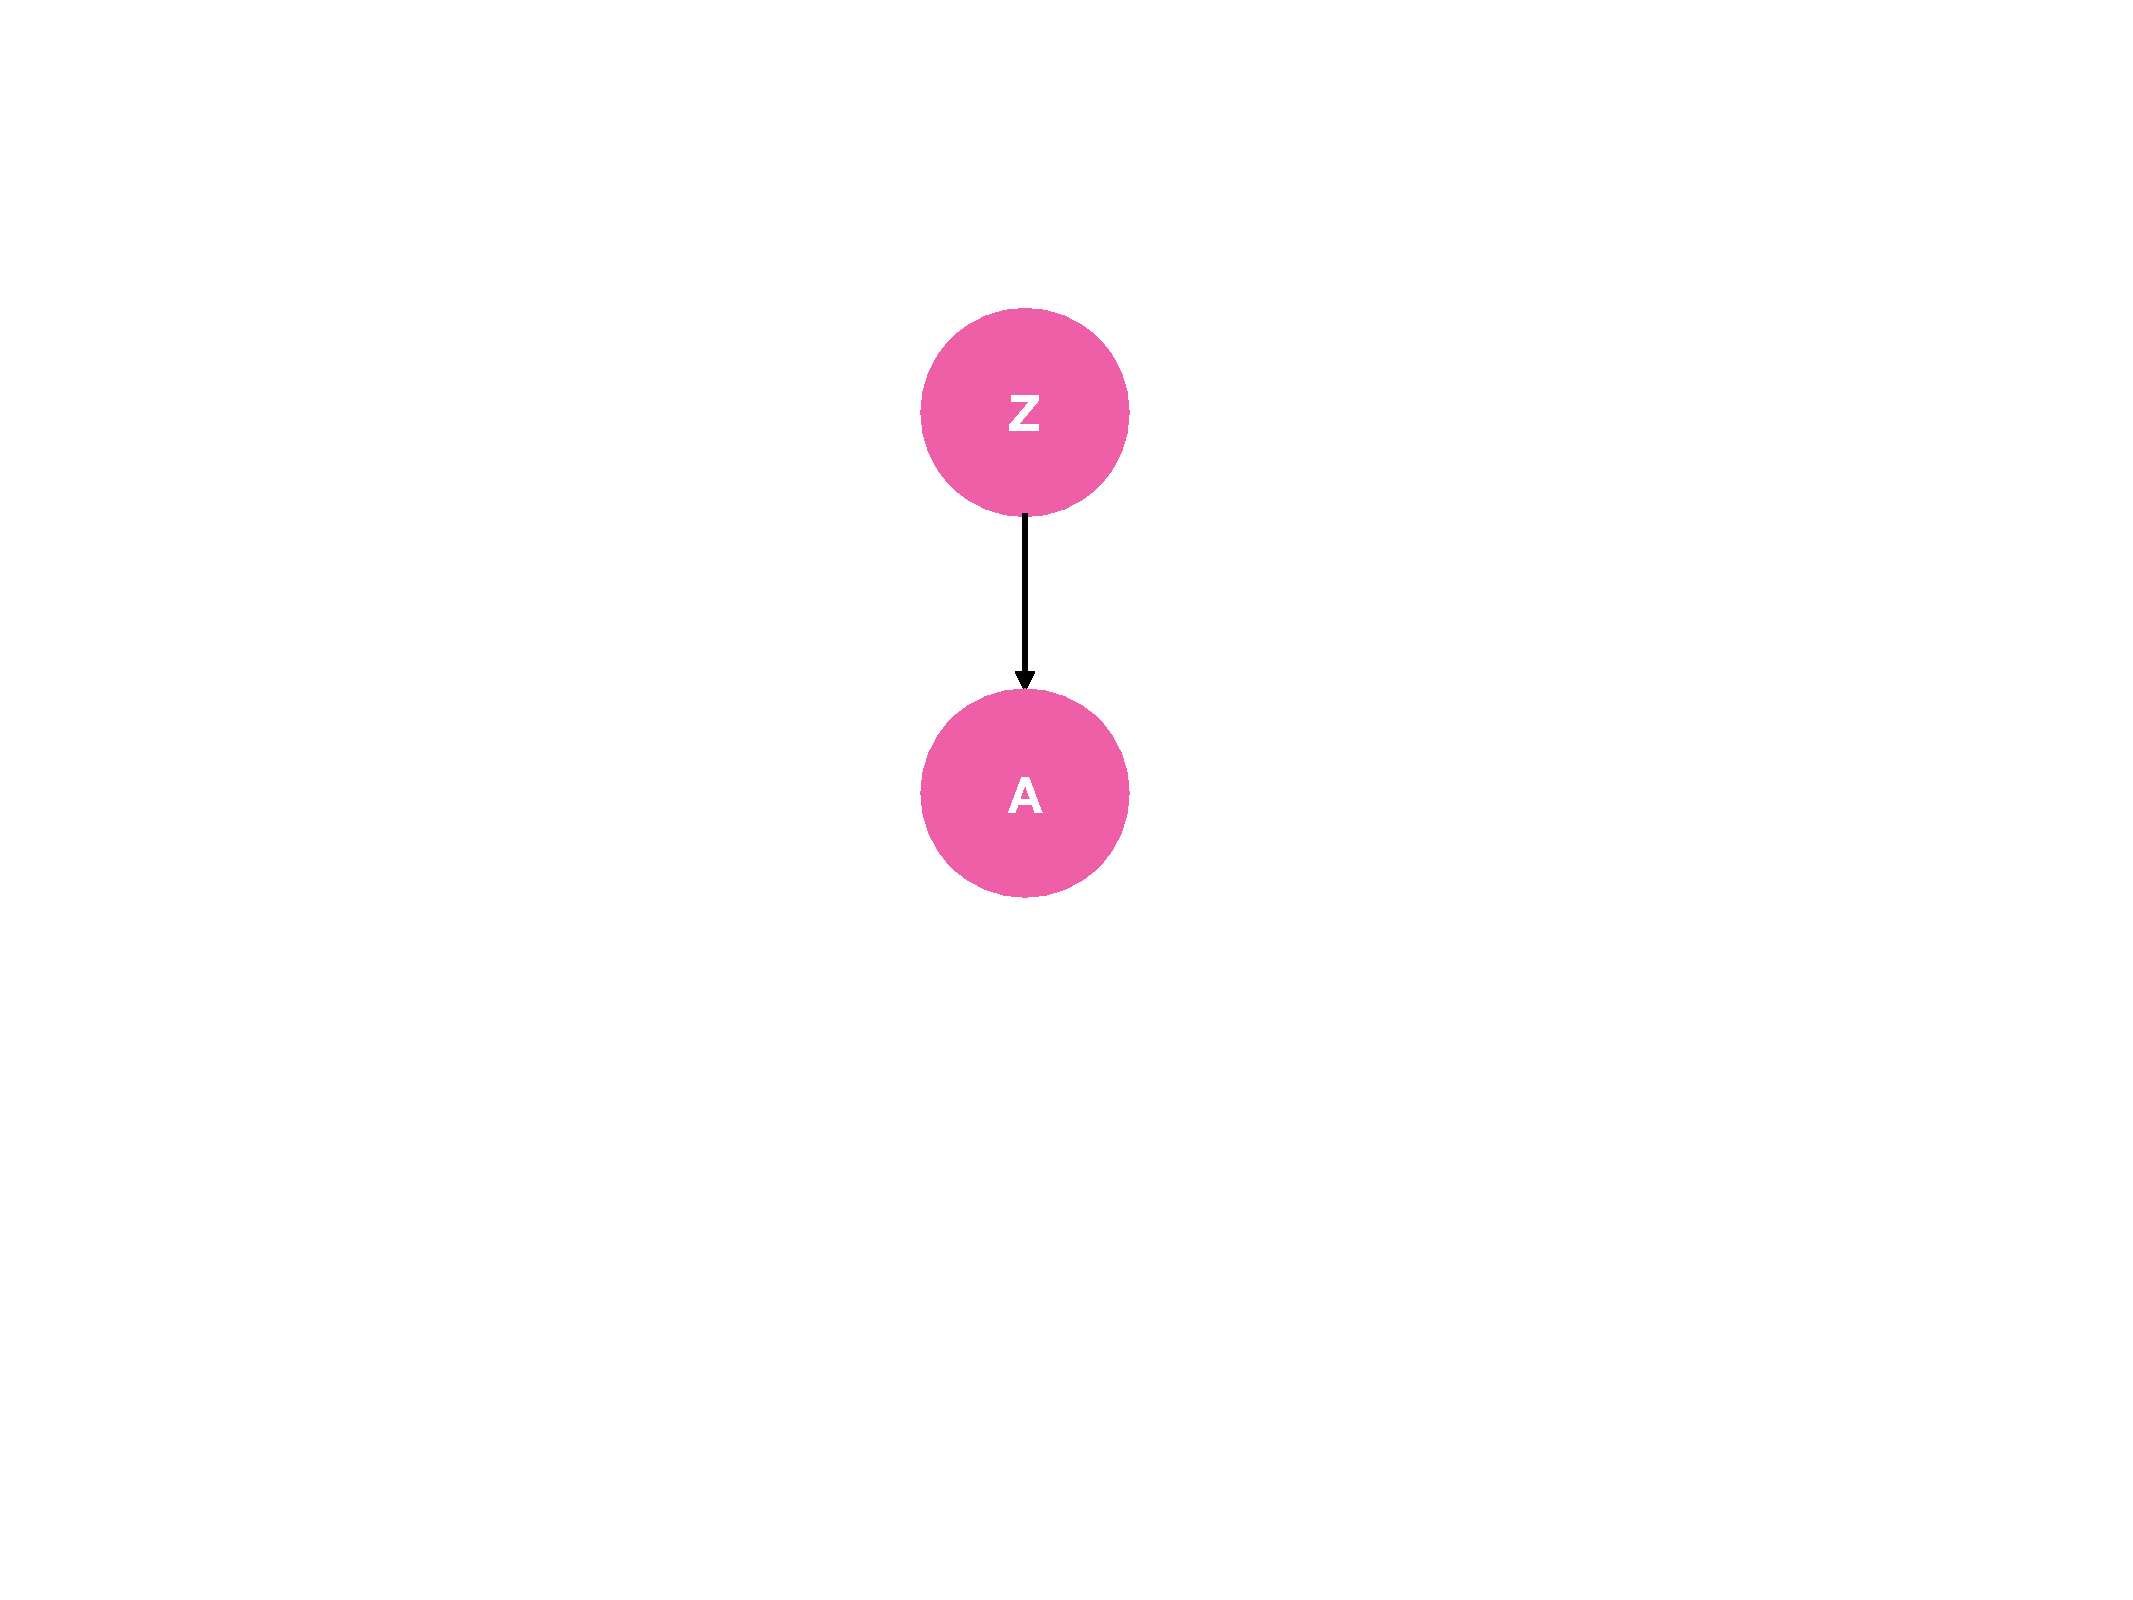
\includegraphics[scale=0.3]{SBMGraphical}
\caption{{\bf SBM Graphical Model.} A graphical model is used to model the dependency between the node-to-community assignments, ${\bf z}$ and the observed network adjacency matrix, ${\bf A}$.}
\label{fig:graphical}
\end{center}
\end{figure}

Using the factorization rules described in section \ref{pgm}, we can specify the complete data log likelihood between ${\bf z}$ and ${\bf A}$ as,

\begin{equation}
\log P({\bf z},{\bf A})=\log(P({\bf A} \mid {\bf z}))+\log(P({\bf z}))
\end{equation}

To further specify these communities, we will define additional notation. First, let ${\boldsymbol \Pi}_{K \times K}=\{\pi_{ij}\}$ be the matrix that specifies the within and between community edge probabilities. Using this information, we can model the probability of an edge existing between nodes $i$ and $j$ as,

\begin{equation}
P(A_{ij}=1)\sim \text{Bernoulli}(\Pi_{z_{i},z_{j}})
\end{equation}

We let $Z_{i}=\{Z_{i1},Z_{i2}, \dots Z_{ik}\}$ be a collection of binary indicators where $Z_{ik}$ is 1 $i$ belongs to community $k$ and 0 otherwise, We also let $\alpha_{k}$ be the probability that a node belongs to community $k$. With all of this information, we can write down each term of the complete data likelihood.

First,

\begin{equation}
\log(P({\bf Z}))=\sum_{i}\sum_{k}Z_{ik}\log(\alpha_{k}).
\end{equation}

Next,

\begin{equation}
\log(P({\bf A} \mid {\bf Z}))=\sum_{i\ne j}\sum_{k< l}Z_{ik}Z_{il}[a_{ij}\log (\Pi_{kl})+(1-a_{ij})\log(1-\Pi_{kl})]
\end{equation}

Optimizing the parameters of this incomplete data log likelihood requires computing the posterior $P({\bf z} \mid {\bf A})$ but as shown by \cite{dudin} is intractable. To address this issue, the posterior can be recast using a factorized approximation. This is accomplished by optimizing a lower bound of $\mathcal{L}({\bf A})$. We let $\mathcal{R}_{A}$ be an approximation of the posterior, $P({\bf z} \mid {\bf A})$. To optimize the lower bound of $\log \mathcal{A}$, we seek the $\mathcal{R}_{A}$ that is as close as possible to $P({\bf z} \mid {\bf A})$. In other words, we define the lower bound of $\mathcal{L}({\bf A})$ as $\mathcal{T}(\mathcal{R}_{A})$, with,

\begin{equation}
\mathcal{T}(\mathcal{R}_{A})=\log \mathcal{L}({\bf A})-\text{KL}[\mathcal{R}_{A}(\bf z), P({\bf z} \mid {\bf A})].
\end{equation}

Here KL denoted the Kullback-Leibler divergence (KL divergence) and the best approximation will be the value that makes the KL divergence the smallest. Jaakkola \emph{et al.}, present a mean field approximation for the posterior distribution \cite{jakk} as,

\begin{equation}
\mathcal{R}_{A}({\bf z})=\prod_{i}h(Z_{i};{\boldsymbol \tau}_{i}).
\end{equation}

Here ${\boldsymbol \tau}=(\tau_{i1}, \dots, \tau_{iK})$ and $\tau_{ik}$ is the approximation that node $i$ belongs to community $k$, or $P(Z_{ik}=1 \mid {\bf A})$. Furthermore, $h(\cdot;{\boldsymbol \tau}_{i})$ denotes the multinomial distribution with parameter ${\boldsymbol \tau}$. 

Daudin \cite{dudin} \emph{et al.}, show that the optimal estimate for $\tau_{ik}$ denoted $\hat{\tau}_{ik}$ satisfies

\begin{equation}
\hat{\tau}_{ik} \propto \alpha_{k}\prod_{j \ne i}\prod_{l}[\theta_{z_{i},z_{j}}^{a_{ij}}(1-\theta_{z_{i},z_{j}})^{1-a_{ij}}]^{\hat{\tau}_{ik}}.
\end{equation}

Here, $\alpha_{k}$ notes the probability that a node belongs to community $k$. Furthermore, after computing the set of variational parameters, the updates for ${\boldsymbol \alpha}$ and ${\boldsymbol \theta}$ that maximize $\mathcal{T}(\mathcal{R}_{A})$ are also shown by Daudin \emph{et al.,} \cite{dudin} to be,

\begin{equation}
\hat{\alpha}_{k}=\frac{1}{n}\sum_{i}\hat{\tau}_{ik}  \hspace{.5in}  {\theta}_{ql}=\sum_{i \ne j}\hat{\tau}_{iq}\hat{\tau}_{jl}a_{ij}/\sum_{i \ne j}\hat{\tau}_{iq}\hat{\tau}_{jl}
\end{equation}

We have presented this variational approach for performing SBM parameter inference and likelihood optimization because this approach was appropriate for the work presented in this thesis. Variational inference is just one approach that can be applied to learn model parameters and was but a study by  Zhang \emph{et al.} \cite{comp} also show that belief propgation is very effective for this task \cite{belief}. Briefly, belief propagation is a message passing algorithm for parameter inference in probabilistic graphical models. Given that parameter learning offer requires computing marginal distributions for a set of variables with a very large number of possible configurations, belief propagation uses the graphical model to reduce the complexity of the problem.  Using the belief propagation to infer latent node-to-community assignments and update the model parameters was shown to perform superperior to the variational appromixation


This formulation of the problem and parameter optimization procedure works well and converges quickly for networks that have assortative community structures and a homogenous degree distribution. We will now explore how this classic formulation of the SBM can be modified to enable a broader application for a variety of networks.

\subsection{Variants to the Classic Stochastic Block Model}

The introduced stochastic block model is the most vanilla version in that it makes the assumption that the network is unweighted, each node is assigned to only one community. The introduced model also does not account for issues that may arise from degree heterogeneity (i.e. a large disparity in node degree in sets of nodes).  Here, we will briefly discuss the approaches that adapt the stochastic block model to handle these issues and assumptions. 

{\bf Edge Weights}

\indent The majority of the stochastic block model literature considers unweighted networks simply because describing a probabilistic model to handle both edge existence and edge weight is a challenging task. In the classic stochastic block model, we are simply modeling whether an edge exists based on the inferred community memberships of the edge stubs. Since edge weights can come in a variety of forms (real-valued, count, etc.), it is difficult to immediately decide what distribution the edge weights should follow. In the past few years, this issue has been tackled in two papers \cite{aicher,peix}.

\indent First, Aicher \emph{et al.} developed a model and associated inference technique, for the weighted stochastic block model. Here, edge weights can be modeled by any exponential family distribution. The authors use a mixing parameter that allows for the control of the use of edge existence versus edge weights when learning node-to-community assignments. This method requires having an estimate of the number of communities, $K$, but the paper provides an approach to use Bayes' factors between two competing values of $K$ to determine which model is a better fit.The inference for fitting this model is performed through a variational bayes approach \cite{vBayes}.

\indent To avoid having intuition about $K$, Peixoto \cite{peix} developed a non parametric bayesian approaches that is capable of inferring $K$ with no prior knowledge. The assumption of the model is also slightly different and assumes a hierarchical structure between communities. The inference is achieved through MCMC sampling. 

{\bf Degree Heterogeneity}\\
\indent Based on the variety of network structures and types, the assumption that the classic stochastic block model is an appropriate model for the data is often invalid. That is, for some networks, the fitted model may not actually be a good fit for the data. Work by Karrer \emph{et al.}, introduced a simple extension to the classic stochastic block model, known as the degree corrected stochastic block model, that is informed by degree distribution as a proxy for the network structure. In networks where there is a high disparity between node degree (i.e. many high degree nodes and many low degree nodes), stochastic block models inference tends to partition the nodes intro communities of high degree and low degree nodes. The approach for adapting the SBM to this setting is to learn a $K \times K$ matrix, ${\boldsymbol \theta}$, describing the number of edges between each pair of communities. these counts are modeled as poisson random variables. The likelihood of the observed network under this poisson assumption takes into account node degrees. 

{\bf The restriction of single community membership}\\
\indent As it is often observed in social networks, the assumption that every node belongs to only a single community is restrictive. To address this issue, approaches have been developed to  allow nodes to  participate in a mixture of communities \cite{mixMember} or to overlapping groups \cite{LA}. Airoldi \emph{et al.}, pioneered the development of the mixed membership stochastic block model \cite{mixMember}, where instead of modeling a node's membership in each community in a binary manner, the authors allow a node to belong to multiple communities. The generative process for this approach for modeling the existence of an edge between nodes $p$ and $q$ in a network with $K$ possible communities and ${\boldsymbol \theta}$ representing the between community connection probabilities.

\begin{itemize}
\item For each node $p$, draw a mixed membership vector $\pi_{p}\sim \text{Dirchelet}({\boldsymbol \alpha})$
\item Then for each pair of nodes $(p,q)$, draw ${\bf z}_{p\rightarrow q} \sim \text{Multinomial}(\pi_{p})$, ${\bf z}_{q\rightarrow p} \sim \text{Multinomial}(\pi_{q})$
\item Sample the edge between $p$ and $q$ as, $A_{pq}$, where $A_{pq} \sim \text{Bernoulli}({\bf z}_{q\rightarrow p}^{T}{\boldsymbol \theta}{\bf z}_{q\rightarrow p})$
\end{itemize} 

Following the development of the mixed membership stochastic block model, Latocuhe \emph{et al.} \cite{LA} addressed an important limitation of \cite{mixMember}. Since the probability of an edge between a pair of nodes $p$ and $q$ depends on a single draw of ${\bf z}_{p\rightarrow q}$ and ${\bf z}_{q\rightarrow p}$, the class memberships of nodes $p$ and $q$ towards other nodes in the network are ignored. Moreover, this model adapts the mixed membership stochastic block model to incorporate more structures of the network. 

\section{Affiliation model and inference}


Duis autem vel eum iriure dolor in hendrerit in vulputate velit esse molestie consequat, vel illum dolore eu feugiat nulla facilisis at vero eros et accumsan et iusto odio dignissim qui blandit praesent luptatum zzril delenit augue duis dolore te feugait nulla facilisi. Lorem ipsum dolor sit amet, consectetuer adipiscing elit, sed diam nonummy nibh euismod tincidunt ut laoreet dolore magna aliquam erat volutpat.   

Ut wisi enim ad minim veniam, quis nostrud exerci tation ullamcorper suscipit lobortis nisl ut aliquip ex ea commodo consequat. Duis autem vel eum iriure dolor in hendrerit in vulputate velit esse molestie consequat, vel illum dolore eu feugiat nulla facilisis at vero eros et accumsan et iusto odio dignissim qui blandit praesent luptatum zzril delenit augue duis dolore te feugait nulla facilisi.   

Nam liber tempor cum soluta nobis eleifend option congue nihil imperdiet doming id quod mazim placerat facer


\chapter{Community Detection in multilayer networks}

\chapter{A multilayer stochastic block model}

\section{Fitting a common stochastic block model to all network layers}

\section{Strata multilayer stochastic block model}

\section{Parameter learning}

\section{A clustering-based fitting approach}

\section{Synthetic examples}

\section{Detectability limits}

\section{Human microbiome project example}

\section{Comparison to reducibility}

\chapter{Network compression}

\chapter{Network compression for community detection with super nodes}
\section{Super pixel pre-processing of images}
\section{Super node pre-processing for networks}
\section{2-Core decomposition approach for selecting seeds as community centers}
\section{Creating a super node network representaion}
\section{Social network data examples}
\section{Benefits of a compressed representation: run time, variability, neighborhood smoothing}

\chapter{Attributed networks and community detection}
\section{Examples of attributed networks}
\section{Models and inference for attributed networks}
\section{Alignment of attributes with communities}

\chapter{An attributed stochastic block model}
\section{Approaches to an attributed stochastic block model}
\section{A model of conditional independence between attributes and connectivity}
\section{Learning the model parameters}
\section{Example on a synthetic attributed network}
\section{Detectability limits in attributed networks}
\section{Case studies for attributed networks}
\section{Attributed SBM in link prediction}
\section{Attributed SBM in collaborative filtering}

\chapter{Software}
\section{sMLSBM}
\section{Super node representations for a network}
\section{Attributed stochastic block model}

\chapter{Conclusion and future work}


% Bibliography
\clearpage
\phantomsection

{\def\chapter*#1{} % suppress bibliograph header.
\begin{singlespace}
\addcontentsline{toc}{chapter}{BIBLIOGRAPHY}
\begin{center}
\Large \textbf{BIBLIOGRAPHY}
\vspace{17pt}
\end{center}

\bibliographystyle{apalike}
\bibliography{dissBib}
\end{singlespace}
}





\end{document}
